\documentclass{standalone}
\usepackage{tikz}
\usepackage{ctex,siunitx}
\setCJKmainfont{Noto Serif CJK SC}
\usepackage{tkz-euclide}
\usepackage{amsmath}
\usepackage{wasysym}
\usetikzlibrary{patterns, calc}
\usetikzlibrary {decorations.pathmorphing, decorations.pathreplacing, decorations.shapes,}
\begin{document}
\small
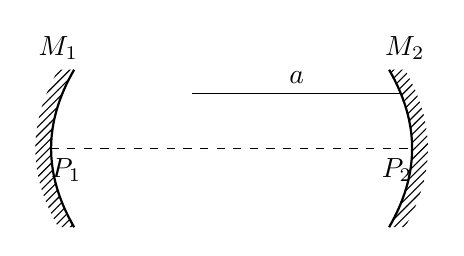
\begin{tikzpicture}[>=latex,scale=1.0]
  \fill [pattern=north east lines] (-2,-1)--(-2.2,-1) to [bend left=30] (-2.2,1) --(-2,1) to [bend left=-30]
  (-2,-1);
\draw [thick](-2,1) to [bend left=-30] (-2,-1);

\fill [pattern=north east lines] (2,-1)--(2.2,-1) to [bend left=-30] (2.2,1) --(2,1) to [bend left=30](2,-1);
\draw [thick](2,1) to [bend left=30] (2,-1);
\draw [dashed] (-2.3,0)--(2.3,0);
\node at (-2.1,0)[below]{$P_1$};\node at (2.1,0)[below]{$P_2$};
\node at (-2.2,1)[above]{$M_1$};\node at (2.2,1)[above]{$M_2$};
\draw (-.5,.7)--node[above]{$a$}(2.15,.7);
\end{tikzpicture}
\end{document}